\section{*应用：乘积空间的上同调环}
\sourcepage{435--436}
上一节定义了上同调叉积，并用它得到上同调的 Künneth 定理。本节考察叉积的一些性质，并用来研究上同调的环结构。先对环 $R$ 系数的叉积（定义 7.10.4）陈述结论，再说明这些结论在多大程度上也适用于 $\Z,G$ 系数的叉积（定义 7.10.5）。设 $X,Y$ 是拓扑空间。

\entry{定义}{7.11.1}叉积是上同调同态 $\Theta$ 与 $\nu^*$ 的复合。这两个同态分别由上链映射 $\theta$ 和 $\overline\nu$ 诱导，因此叉积由 $\overline\nu\circ\theta$ 诱导。相应地定义
\[
c^p\times c^q=\overline\nu\theta(c^p\otimes c^q),
\]
称为\emph{上链叉积}。它诱导上同调叉积。

若 $m=p+q$，$T:\Delta_m\to X\times Y$，则
\begin{align*}
\langle c^p\times c^q,T\rangle
&=\langle\theta(c^p\otimes c^q),\nu(T)\rangle\\
&=\sum_{i=0}^m\langle c^p,\pi_1T\ell(\epsilon_0,\ldots,\epsilon_i)\rangle
\langle c^q,\pi_2T\ell(\epsilon_i,\ldots,\epsilon_m)\rangle.
\end{align*}
和式中只有 $i=p$ 的项可能非零。因此得到：

\entry{引理}{7.11.2}上链叉积由下式给出：
\[
\langle c^p\times c^q,T\rangle=
\langle c^p,\pi_1T\ell(\epsilon_0,\ldots,\epsilon_p)\rangle
\langle c^q,\pi_2T\ell(\epsilon_p,\ldots,\epsilon_m)\rangle.
\]
这个结论也适用于 $\Z,G$ 系数。它表示，$c^p\times c^q$ 在 $T$ 上的值，等于 $c^p$ 在 $T$ 第一分量的前面上的值，乘以 $c^q$ 在第二分量的后面上的值。

\entry{定理}{7.11.3}叉积具有以下性质。
\begin{enumerate}[label=(\alph*)]
\item 若 $\lambda:X\times Y\to Y\times X$ 交换坐标，则
\[\lambda^*(\beta^q\times\alpha^p)=(-1)^{pq}\alpha^p\times\beta^q.\]
\item 在 $H^*(X\times Y\times Z;R)$ 中，
\[(\alpha\times\beta)\times\gamma=\alpha\times(\beta\times\gamma).\]
\item 设 $\pi_1,\pi_2$ 是两个投影，$1_X,1_Y$ 是相应上同调环的单位元，则
\[\pi_1^*(\alpha^p)=\alpha^p\times1_Y,\qquad \pi_2^*(\beta^q)=1_X\times\beta^q.\]
\end{enumerate}

\textbf{证明：}(a) 定义
\[
\omega:(\mathcal S(X)\otimes\mathcal S(Y))_m\to(\mathcal S(Y)\otimes\mathcal S(X))_m,
\quad\omega(c_p\otimes c_q)=(-1)^{pq}c_q\otimes c_p.
\]
可检验 $\omega$ 是链映射；若没有符号 $(-1)^{pq}$，就不再是链映射。我们要证明
\[
\omega\nu\simeq\nu\lambda_\#.
\]
\sourcepage{437}
已知 $\lambda_\#$ 和 $\nu$ 保持增广，且对于连续映射诱导的同态是自然的；$\omega$ 也有这些性质。考虑函子
\[
\begin{array}{ll}
G(X,Y)=\mathcal S(X\times Y),&G(f,g)=(f\times g)_\#,\\
G'(X,Y)=\mathcal S(Y)\otimes\mathcal S(X),&G'(f,g)=g_\#\otimes f_\#.
\end{array}
\]
已经证明它们相对于模型族 $\{(\Delta_p,\Delta_q)\}$ 自由且无环。因此 $G$ 到 $G'$ 的任意两个保持增广的自然变换自然链同伦。$\omega\nu$ 和 $\nu\lambda_\#$ 正是这样的自然变换，所以链同伦。

对偶化上述关系，并定义
\[
\eta(c^q\otimes c^p)=(-1)^{pq}c^p\otimes c^q.
\]
直接检验得到
\[\theta\eta=\overline\omega\theta.\]
另一方面，由刚证明的链同伦得到
\[\overline\nu\,\overline\omega\simeq\lambda^\#\overline\nu.\]
因此，由 $\eta,\theta,\overline\nu,\lambda^\#$ 组成的对偶图在上同调上交换，从而得到 (a)。

(b)、(c) 也可以用无环模型论证，但用引理 7.11.2 的上链公式更容易。将该公式应用两次，立即得到 (b)。

为验证 (c)，取代表 $\alpha^p$ 的上闭链 $z^p$，并令 $z^0$ 为 $Y$ 上在每个奇异零单形上取值 $1$ 的上闭链。$\alpha^p\times1_Y$ 由 $z^p\times z^0$ 代表。对 $T:\Delta_p\to X\times Y$，有
\begin{align*}
\langle z^p\times z^0,T\rangle
&=\langle z^p,\pi_1T\ell(\epsilon_0,\ldots,\epsilon_p)\rangle
\langle z^0,\pi_2T\ell(\epsilon_p)\rangle\\
&=\langle z^p,\pi_1T\rangle=\langle\pi_1^\#z^p,T\rangle.
\end{align*}
所以 $\alpha^p\times1_Y=\pi_1^*(\alpha^p)$。另一个等式同理。\hfill$\square$

经过适当解释，三种性质也都适用于另一种系数的叉积。(a) 中右端取 $\Z,G$ 系数，左端相应交换系数次序；(b) 在三个系数群中两个为 $\Z$、一个为 $G$ 时成立；(c) 的第一个等式在 $1_Y\in H^0(Y)$、$\alpha^p\in H^p(X;G)$ 时成立，因为此时 $\alpha^p\times1_Y\in H^p(X\times Y;G)$，等式有意义。另一个等式也作同样解释。

\sourcepage{438}
上链叉积公式与杯积公式十分相似，这提示二者之间存在关系。下一定理给出这种关系。

\entry{定理}{7.11.4}设 $d:X\to X\times X$ 为对角映射 $d(x)=(x,x)$，则对两种系数的叉积都有
\[d^*(\alpha^p\times\beta^q)=\alpha^p\smile\beta^q.\]

\textbf{证明：}取代表上闭链 $z^p,z^q$。对奇异单形 $T:\Delta_{p+q}\to X$，令 $m=p+q$，则
\begin{align*}
\langle d^\#(z^p\times z^q),T\rangle
&=\langle z^p\times z^q,dT\rangle\\
&=\langle z^p,\pi_1dT\ell(\epsilon_0,\ldots,\epsilon_p)\rangle
\langle z^q,\pi_2dT\ell(\epsilon_p,\ldots,\epsilon_m)\rangle\\
&=\langle z^p\smile z^q,T\rangle,
\end{align*}
这里使用了 $\pi_1d=i_X=\pi_2d$。\hfill$\square$

这一定理归功于 Lefschetz。它说明为何上同调具有环结构，而同调没有相应的这种结构。同调和上同调都有叉积，但只有在上同调中，才能把叉积与对角映射诱导的同态复合。在同调中，相应的图为
\[
H_p(X)\otimes H_q(X)\xrightarrow{\times}H_{p+q}(X\times X)
\xleftarrow{d_*}H_{p+q}(X),
\]
其中 $d_*$ 的方向不允许作所需的复合！

\entry{推论}{7.11.5}两种系数的杯积均满足反交换律
\[\alpha^p\smile\beta^q=(-1)^{pq}\beta^q\smile\alpha^p.\]

\textbf{证明：}设 $\lambda:X\times X\to X\times X$ 交换坐标。由于 $\lambda d=d$，
\begin{align*}
\alpha^p\smile\beta^q
&=d^*(\alpha^p\times\beta^q)
=d^*\lambda^*(\alpha^p\times\beta^q)\\
&=(-1)^{pq}d^*(\beta^q\times\alpha^p)
=(-1)^{pq}\beta^q\smile\alpha^p.
\end{align*}
\translatornote{原文此处有将 $pq$ 印作 $pg$、并在中间一步把叉积写作杯积的排印错误；这里按定义写出。}\hfill$\square$

下面计算乘积空间上同调中的杯积。

\entry{定理}{7.11.6}在 $H^*(X\times Y;R)$ 中，
\[
(\alpha\times\beta)\smile(\alpha'\times\beta')
=(-1)^{pq}(\alpha\smile\alpha')\times(\beta\smile\beta'),
\qquad p=\dim\alpha',\quad q=\dim\beta.
\]

\sourcepage{439}
\textbf{证明：}设 $\pi_1,\pi_2$ 为投影。

第一步：先证明 $\beta$ 和 $\alpha'$ 都为各自环的单位元时的公式。设 $z^p,z^q$ 分别代表 $\alpha,\beta'$。由上链叉积公式，
\begin{align*}
\langle z^p\times z^q,T\rangle
&=\langle z^p,\pi_1T\ell(\epsilon_0,\ldots,\epsilon_p)\rangle
\langle z^q,\pi_2T\ell(\epsilon_p,\ldots,\epsilon_m)\rangle\\
&=\langle\pi_1^\#z^p,T\ell(\epsilon_0,\ldots,\epsilon_p)\rangle
\langle\pi_2^\#z^q,T\ell(\epsilon_p,\ldots,\epsilon_m)\rangle\\
&=\langle\pi_1^\#z^p\smile\pi_2^\#z^q,T\rangle.
\end{align*}
因此
\[\alpha\times\beta'=\pi_1^*(\alpha)\smile\pi_2^*(\beta')
=(\alpha\times1_Y)\smile(1_X\times\beta').\]

第二步：证明 $\beta,\beta'$ 都为单位元时的公式。杯积的自然性给出
\[\pi_1^*(\alpha)\smile\pi_1^*(\alpha')=\pi_1^*(\alpha\smile\alpha'),\]
也就是
\[(\alpha\times1_Y)\smile(\alpha'\times1_Y)=(\alpha\smile\alpha')\times1_Y.\]
对第二因子也有同样结论。

第三步：一般情形由前两步及反交换律得到：
\begin{align*}
(\alpha\times\beta)\smile(\alpha'\times\beta')
&=(\alpha\times1_Y)\smile(1_X\times\beta)\smile(\alpha'\times1_Y)\smile(1_X\times\beta')\\
&=(-1)^{pq}(\alpha\times1_Y)\smile(\alpha'\times1_Y)\smile(1_X\times\beta)\smile(1_X\times\beta')\\
&=(-1)^{pq}(\alpha\smile\alpha')\times(\beta\smile\beta').
\end{align*}
\hfill$\square$

这一定理使我们能够由两个因子的杯积，计算乘积空间上同调环中某些元素的杯积。当上同调 Künneth 定理适用时，可以更正式地表述为定理 7.11.8。

\entry{定义}{7.11.7}在 $H^*(X;R)\otimes_R H^*(Y;R)$ 上定义环结构：对 $\beta\in H^p(Y;R)$、$\alpha'\in H^q(X;R)$，令
\[
(\alpha\otimes\beta)\smile(\alpha'\otimes\beta')
=(-1)^{pq}(\alpha\smile\alpha')\otimes(\beta\smile\beta').
\]
读者可检验此运算定义良好，且满足环公理；特别是其中的符号使结合律成立。

\sourcepage{440--441}
\entry{定理}{7.11.8}若所有 $H_i(X)$ 都有限生成，则叉积给出环单同态
\[\times:H^*(X)\otimes H^*(Y)\longrightarrow H^*(X\times Y).\]
若 $F$ 是域，则
\[\times:H^*(X;F)\otimes_F H^*(Y;F)\longrightarrow H^*(X\times Y;F)\]
是代数同构。

\entry{例}{7.11.9}考虑 $S^n\times S^m$ 的上同调环，其中 $n,m\ge1$。取生成元 $\alpha^n\in H^n(S^n)$、$\beta^m\in H^m(S^m)$。则 $H^*(S^n\times S^m)$ 是秩为 $4$ 的自由群，基为
\[1\times1,\quad\alpha\times1,\quad1\times\beta,\quad\alpha\times\beta.\]
正维元素之间唯一的非平凡乘积（以及由反交换律得到的乘积）是
\[(\alpha\times1)\smile(1\times\beta)=\alpha\times\beta.\]

特别地，$n=m=1$ 时空间是环面，这就是例 5.10.5 中已计算的上同调环。下面把这些类画出来。用图 7.11.1 中的通常方式表示环面。设 $X$ 是子空间 $abca$，则其一维上同调生成元 $\alpha$ 由上闭链 $x^1=[b,c]^*$ 代表。投影 $\pi_1$ 是单纯映射，因此 $\pi_1^\#(x^1)$ 就是图中的环面上闭链 $w^1$，代表 $\alpha\times1$。类似地，图 7.11.2 的上闭链 $z^1$ 代表 $1\times\beta$，其中 $\beta$ 由空间 $Y=adea$ 上的 $[d,e]^*$ 代表。杯积 $(\alpha\times1)\smile(1\times\beta)=\alpha\times\beta$ 生成 $H^2(T)$。

\begin{figure}[htbp]\centering
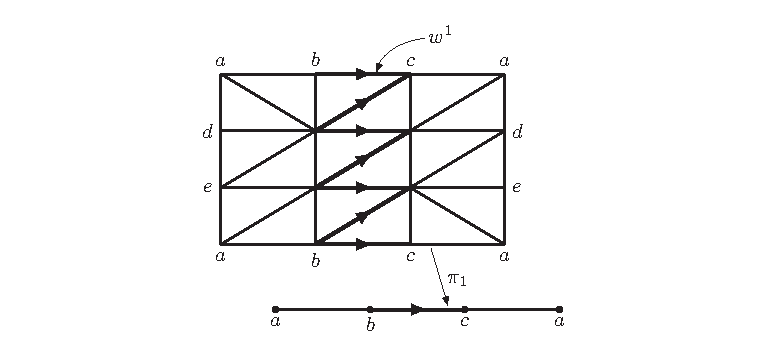
\includegraphics[width=.86\textwidth]{figures/7-11-1.pdf}
\caption*{图 7.11.1}
\end{figure}
\begin{figure}[htbp]\centering
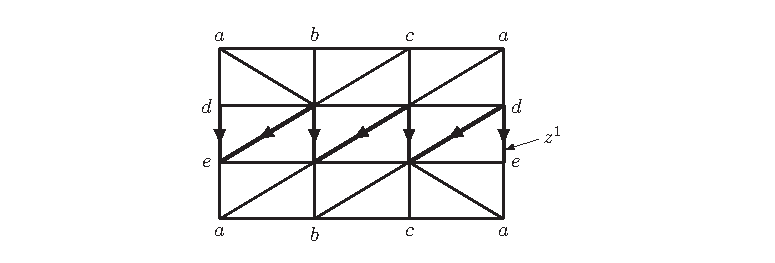
\includegraphics[width=.86\textwidth]{figures/7-11-2.pdf}
\caption*{图 7.11.2}
\end{figure}

\entry{例}{7.11.10}考虑 $P^2\times P^2$ 的 $\Z/2$ 系数上同调环。设 $\alpha\in H^1(P^2;\Z/2)$ 是非零元，则 $\alpha^2=\alpha\smile\alpha\ne0$（见第 5.10 节习题）。由定理 7.11.8，$H^*(P^2\times P^2;\Z/2)$ 是九维向量空间，各维的基如下：
\[
\begin{array}{c|l}
0&1\times1\\
1&\alpha\times1,\quad1\times\alpha\\
2&\alpha^2\times1,\quad\alpha\times\alpha,\quad1\times\alpha^2\\
3&\alpha^2\times\alpha,\quad\alpha\times\alpha^2\\
4&\alpha^2\times\alpha^2
\end{array}
\]
其乘法表容易写出。系数域为 $\Z/2$，所以不涉及符号问题。

下面的定义将在习题 3 中使用。

\entry{定义}{7.11.11}若 $M,N$ 是连通 $n$ 维流形，分别从中去掉一个开 $n$ 维球，再沿边界把剩余部分粘合，所得空间称为\emph{连通和}（connected sum），记为 $M\mathbin{\#}N$。对习题 3 中的流形，所得流形在同胚意义下定义良好；一般情形还必须考虑“定向”问题。

\sourcepage{441--442}
\subsection*{习题}
\begin{enumerate}
\item \begin{enumerate}[label=(\alph*)]
\item 设 $A\subset X$、$B\subset Y$。证明：若 $\{X\times B,A\times Y\}$ 是切除偶，则对通常采用的系数，存在相对上同调叉积
\[H^p(X,A)\otimes H^q(Y,B)\xrightarrow{\times}
H^{p+q}(X\times Y,(X\times B)\cup(A\times Y)).\]
\item 对相对杯积证明定理 7.11.4 和推论 7.11.5。
\end{enumerate}
\item \begin{enumerate}[label=(\alph*)]
\item 按本节方式定义叉积，并用 $\alpha\smile\beta=d^*(\alpha\times\beta)$ 定义杯积，其中 $d$ 是对角映射。利用叉积性质证明杯积双线性、满足结合律，且 $\{z^0\}$ 起单位元作用。
\item 按第 5.9 节定义杯积，再用 $\alpha\times\beta=\pi_1^*(\alpha)\smile\pi_2^*(\beta)$ 定义叉积，其中 $\pi_1,\pi_2$ 是投影。利用杯积性质证明叉积双线性、满足结合律，并证明
\[\pi_1^*(\alpha)=\alpha\times1_Y,\qquad\alpha\smile\beta=d^*(\alpha\times\beta).\]
\end{enumerate}
\item 计算下列上同调环：
\begin{enumerate}[label=(\alph*)]
\item $H^*(S^1\times S^1\times S^3)$。
\item $H^*((T\mathbin{\#}T)\times S^3)$，其中 $T$ 是环面。
\item $H^*((S^1\times S^5)\mathbin{\#}(S^2\times S^4))$。
\end{enumerate}
\item 设 $M$ 为紧致连通 $n$ 维流形，$H_n(M)\cong\Z$。利用上一题结果，对杯积
\[H^k(M)\otimes H^{n-k}(M)\longrightarrow H^n(M)\]
提出一个猜想。
\item 设 $S$ 为 Klein 瓶，$T$ 为环面。计算：
\begin{enumerate}[label=(\alph*)]
\item $H^*(T\times S)$；\item $H^*(T\times S;\Z/2)$。
\end{enumerate}
\item 验证定理 7.11.3(a) 证明中的 $\omega$ 是链映射。
\end{enumerate}
